\documentclass[10pt]{article}
\usepackage[marginparsep=1em]{geometry}
\geometry{lmargin=.50in,rmargin=.50in,bmargin=.50in,tmargin=.75in}
\usepackage[utf8]{inputenc}
\usepackage{amsmath}
\usepackage{amsfonts}
\usepackage{amssymb}
\usepackage{graphicx}
\usepackage{fancyhdr}
\usepackage{hyperref}
\usepackage{listings, xcolor}
\lstdefinestyle{java}{
    language=Java,
    frame = trBL,    
    firstnumber=last,
    basicstyle=\small\ttfamily,
    keywordstyle=\color{blue},
    commentstyle=\color{green},
    stringstyle=\color{red},
    numbers=left,
    numberstyle=\tiny,
    tabsize=2,
    breaklines=true,
}
\pagestyle{fancy}
\fancyhf{}
\lhead{Sara Prettyman}
\rhead{CS 2420}
\chead{\textbf{DATA STRUCTURES \& ALGORITHMS}}
\lfoot{Page \thepage}
\rfoot{Utah State University}
\title{Final Review}
\author{Sara Prettyman}
\date{\today}
\begin{document}
\maketitle
\begin{center}
    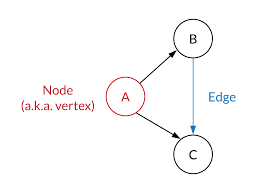
\includegraphics{review.png}
\end{center}
\tableofcontents
\newpage


\begin{center}
    \section{Unit 8: Introduction to Graphs}
\end{center}

\subsection{Introduction to Graphs}
\subsubsection{Introduction to Graphs}
\begin{itemize}
    \item A graph is a finite set of nodes with edges between nodes
    \item A graph G is a structure (V,E) consisting of:\\
          \indent- a finite set V called the set of nodes (vertices)\\
          \indent- a set that is a subset of VE
\end{itemize}
\paragraph{Terminology}
\begin{itemize}
    \item What are some characteristics of a binary tree? Rigid structure where each node has a single node that points to it.
    \item GRAPH - set of vertices/nodes and set of edges/arcs
          \begin{itemize}
              \item More formally, as graph is a ordered pair of finite set V and E
              \item V is the set of vertices
              \item E is the set of edges
              \item If edges have weight, termed weighted graph
              \item If edges have direction, (can traverse from A to B but not B to A)\\
                    \indent -called directed graph otherwise undirected
          \end{itemize}
    \item SUCCESSOR  - the follows relationship of a directed graph
    \item PREDECESSOR  - the precedes relationship in a directed graph
    \item DEGREE - the number of edges incident to or touching a vertex
          \begin{itemize}
              \item IN-DEGREE - the number of edges coming into a vertex (digraph only)
              \item OUT-DEGREE - the number of edges going out of a vertex. (digraph only)
          \end{itemize}
    \item Diagraph - another name for a directed graph
    \item CONNECTED - a graph is connected if you can get from a node to every other node following edges.
    \item When (x,y) is an edge we say: x is adjacent to y, y is adjacent from x.
\end{itemize}
\paragraph{Intuition}
\begin{itemize}
    \item Nodes represent entities like people and cities
    \item Edges represent relationships between entities x and y, for instance x likes y.
\end{itemize}
\newpage

\subsubsection{Graph Representations}
\begin{itemize}
    \item For graphs to be computationally useful, they have to be conveniently represented in programs.
    \item Two common representations are adjacency matrix representation, adjacency list representation.
\end{itemize}

\paragraph{Adjacency Matrix Representation}
\begin{itemize}
    \item Each graph of n nodes is represented by an nxn matrix A, that is, a two dimensional array A.
    \item The nodes are (re)labeled 0,1,2,3,.., n-1. They are given integer labels.
    \item \[A[i][j]=
              \begin{cases}
                  \textrm{true, if (i,j) is an edge} \\
                  \textrm{false, if (i,j) is not an edge.}
              \end{cases}\]
          Like A[0][1], if 0 is connected to 1.
    \item PRO: Simple to implement and easy and fast to tell if a pair is an edge.
    \item CON: No matter how few edges the graph has, it take up O($n^2)$ memory.
    \item The adjacency matrix is a reasonable way to store the graph for the following operations:
          \begin{itemize}
              \item Get successors for node x. (you can just look at row x and see if there is a 1 for each column)
              \item Determine if the graph is connected. (you can use a disjoint set to union all nodes traversed, and in the end if there is only one root node, then it is connected.)
              \item Get predeccessors fo node x. (you can just look at column x and see if there is a 1 for each row)
              \item Determine if there is an edge from node x to node y. (you can just look at A[x][y] and see if it is a 1)s
          \end{itemize}
    \item Time and space complexity:
          \begin{itemize}
              \item Space: O($n^2$) where n is the number of nodes and m is the number of edges
              \item Check if edge (u,v) exist: O(1)
              \item Remove a vertex: O(n)
              \item Adjacency matrices are more efficient for dense graphs with a large number of edges
          \end{itemize}
\end{itemize}
\paragraph{Adjacency List Representation}
\begin{itemize}
    \item A graph of n nodes is represented by a one-dimensional array L of linked list, where\\
          - L[i] is a linked list containing all the nodes adjacent from node i\\
          - The nodes in list L[i] may or may not be in any particular order.
    \item Easy operation is know which nodes follow a value.
    \item Hard to see which edges go from a value. It isn't that hard, just trivial .
    \item Pros: saves space on memory
    \item Cons: it takes time to O(n to look up if a pair of nodes share an edge. Have to search the linked list L[i]
    \item The adjacency list is a reasonable way to store the graph for the following operations:
          \begin{itemize}
              \item Determine if there is an edge from x to y (you can just look at the linked list L[x] and see if y is in the list)
              \item List all edges in the graph (you can just look at each linked list L[i] and print out all the edges)
              \item Get successors of node x (you can just look at linked list L[x] and print out all the nodes)
          \end{itemize}
    \item Time and space complexity:
          \begin{itemize}
              \item Space: O(n+m) where n is the number of nodes and m is the number of edges
              \item Check if edge (u,v) exist: O(degree(u))
              \item Remove a vertex: O(n+m)
              \item Adjacency lists are more efficient for sparse graphs with a small number of edges
          \end{itemize}
\end{itemize}

\subsubsection{Directed vs Undirected Graphs}
\begin{itemize}
    \item An undirected graph is said to be connected if there is a path between every pair of nodes. Otherwise the graph is disconnected, meaning there are nodes riding solo.
    \item If an undirected graph is not connected, then each piece is called a connected component.
    \item If the graph is connected, then the whole graph is one single connected component.
\end{itemize}
\paragraph{Is Connected - Algorithm}
\begin{itemize}
    \item Mark all nodes as unvisited
    \item Select an unvisited node. Make the node as visited.
    \item Recursively visit all nodes reachable from this node - mark each node as visited
    \item Are all nodes visited: yes, connected. no, disconnected.
    \item Adjacency List Representation - Is Connected Code:
          \begin{lstlisting}[style=java]
            // Must add a visited ArrayList to the Graph class
            // Alternatively, add a visited property to the nodes
            
            public boolean isConnected() {
                clearVisitedFlags();
                traverse(0);
                for (int i = 0; i < vertexCount; i++) {
                    if (!visited[i]) return false;
                }
                return true;
            }
            
            public void traverse(int n) {
                if (visited[n]) return;
                visited[n] = true;
                for (EdgeInfo e : adjacencyList.get(n)) {
                    traverse(e.to);
                }
            } 
          \end{lstlisting}
\end{itemize}
\paragraph{Find Connected Components - Algorithm}
\begin{itemize}
    \item Mark all nodes as unvisited.
    \item Initialize component (piece) name to 0
    \item Repeat
          \begin{itemize}
              \item Select an unvisited code: Make the node as visited, make the nodes component
              \item Recursively visit all nodes reachable from this node: make the node as visited, make the nodes component
              \item Increment component name by 1.
          \end{itemize}
\end{itemize}
\paragraph{Strongly and Weakly Connected Components}
\begin{itemize}
    \item  Every pair of vertices are reachable from each other
    \item Graph G is strongly connected if, for every (u, v) in V, there is some path from u to v and some path from v to u
    \item A graph is weakly connected if the underlying undirected graph is connected
    \item Can collapse a Strongly Connected Component (SCC) into a single supernode
\end{itemize}
\paragraph{Subgraph}
\begin{itemize}
    \item Suppose the graph on the left represents one way streets in a town and the nodes represent hotels
    \item Maybe I only care about hotels 0, 1, 3, 6. I can take those nodes and edges between them and talk about the subgraph
    \item Subgraph - a graph that consists of a subset of vertices and all the edges between those vertices
\end{itemize}

\subsubsection{More Terminology}
\textit{Additional Info}
\begin{itemize}
    \item By definition a \textbf{simple graph} does not contain
          \begin{itemize}
              \item Multiple copies of the same edge
              \item \textbf{Self-edges} - edges of the form (a, a); this is also called a loop
                    \begin{itemize}
                        \item Also known as a self-loop; an edge that connects a vertex to itself.
                    \end{itemize}
          \end{itemize}
    \item If we allow multiple edges between the same pair of nodes, it is termed a \textbf{multi-graph}.
          \begin{itemize}
              \item e.g., multiple edges between hotels could represent two different roads between the hotels
          \end{itemize}
    \item Paths
          \begin{itemize}
              \item \textbf{Path } - a sequence of edges
              \item \textbf{Simple Path} - there are no repeated vertices or edges
              \item \textbf{Length of a path} - the sum of the lengths/weights of the edges on the path
          \end{itemize}
    \item Cycle
          \begin{itemize}
              \item A path that begins and ends at the same place
              \item \textbf{Simple Cycle} - a cycle with no repeated vertices; except for the beginning and ending vertex
          \end{itemize}
\end{itemize}
\newpage
\subsubsection{Homework 8.1}
\begin{enumerate}
    \item \textbf{An undirected graph contains a path from every node to every other node. How do we describe this graph?}\\
          \textit{Answer:} A connected graph.
    \item \textbf{In a directed graph, what feature describes a strongly connected component?}\\
          \textit{Answer:} Every pair of vertices are reachable from each other. For every pair of vertices, (u, v) and (v, u), in the component, there exists a directed path that connects them.
    \item \textbf{Consider the following constructor for a graph}\\
          \begin{lstlisting}[style=java]
                Graph(int size) {
                        G = new GraphNode[size];
                        nodeCount = size;
                        for (int i = 0 ; i < size ; i ++) {
                           G[i].name = "A" + i;
                           G[i].nodeID= i;
                           G[i].isVisted = false;
                           G[i].dist = INFINITY;
                        }
                     }
            \end{lstlisting}
          \textbf{What is true about the nodes?}\\
          \textit{Answer:} The nodes are indexed by integers.
    \item \textbf{Consider the following code}\\
          \begin{lstlisting}[style=java]
                public class EdgeInfo {
                        public EdgeInfo(int from, int to){
                            this.from = from;
                            this.to = to;
                    }

                        private int from;        // source of edge
                        private int to;          // destination of edge
                    }

                public class Graph {
                    private int numVertex;
                    private LinkedList<EdgeInfo>[] list;

                    public Graph() {
                        this.numVertex = 0;
                    }

                    public Graph(int numVertex) {
                        this.numVertex = numVertex;
                        list = new LinkedList[numVertex];
                        for (int i = 0; i < numVertex; i++) {
                            list[i] = new LinkedList<EdgeInfo>();
                        }
                    }
                    }

                \end{lstlisting}
          \textbf{What does the following code do?}
          \begin{lstlisting}[style=java]
                    for (int j = 0; j < list[i].size(); j++) {
                        System.out.print(list[i].get(j) + " ");
                    }
                \end{lstlisting}
          \textit{Answer:} Prints out all successors of node i.
    \item \textbf{Consider the following code}\\
          \begin{lstlisting}[style=java]
            public class EdgeInfo {
                    public EdgeInfo(int from, int to){
                        this.from = from;
                        this.to = to;
                }

                    private int from;        // source of edge
                    private int to;          // destination of edge
                }

            public class Graph {
                private int numVertex;
                private LinkedList<EdgeInfo>[] list;

                public Graph() {
                    this.numVertex = 0;
                }

                public Graph(int numVertex) {
                    this.numVertex = numVertex;
                    list = new LinkedList[numVertex];
                    for (int i = 0; i < numVertex; i++) {
                        list[i] = new LinkedList<EdgeInfo>();
                    }
                }
                }

            \end{lstlisting}
          \textbf{What does the following code do?}
          \begin{lstlisting}[style=java]
                public boolean doIt(int i) {
                    for (int j = 0; j < list[i].size(); j++) {
                        if (i == list[i].get(j).to) return true;
                    }
                    return false;
                }
            \end{lstlisting}
          \textit{Answer:} Checks if there is a self-loop from i to i.
\end{enumerate}
\newpage
\subsubsection{Graph Node, Adjacency List Example }
\begin{lstlisting}[style=java]
            import java.util.*;

            class GraphNode {
                public int id;
                public int parent;
                public LinkedList<EdgeInfo> successor;
                public boolean visited;

                public GraphNode(int id) {
                    this.id = id;
                    this.successor = new LinkedList<>();
                    this.parent = -1;
                    this.visited = false;
                }

                public String toString() {
                    StringBuilder sb = new StringBuilder();
                    sb.append(id + ": ");

                    for (var edge : successor) {
                        sb.append(edge.toString());
                    }

                    sb.append("\n");
                    return sb.toString();
                }

                public void addEdge(int v1, int v2, int capacity) {
                    successor.addFirst(new EdgeInfo(v1, v2, capacity));
                }

                public class EdgeInfo {
                    int from;        // source of edge
                    int to;          // destination of edge
                    int capacity;    // capacity of edge

                    public EdgeInfo(int from, int to, int capacity) {
                        this.from = from;
                        this.to = to;
                        this.capacity = capacity;

                    }

                    public String toString() {
                        return "Edge " + from + "->" + to + " (" + capacity + ") ";
                    }
                }
            }

        \end{lstlisting}

\subsection{Graph Traversals}
\subsubsection{Introduction}
\paragraph{Two standard techniques}
\begin{itemize}
    \item Depth First Search (DFS), Breadth First Search (BFS). The nodes of an undirected graph are visited in a systemic  manner so that every node is visited exactly once; both traversals can be performed on a directed graph
    \item  Both BFS and DFS consider an embedded tree\\
          -When a node x is visited, it is labeled as visited, and it is added to the tree\\
          - If the traversal got to node x from node y, y is viewed as the parent of x, and x a child of y
\end{itemize}

\subsubsection{Depth First Search}
\begin{enumerate}
    \item Select an unvisited node x, visit it, and treat as the current node
    \item Find an unvisited neighbor of the current node, visit it, and make it the new current node
    \item If the current node has no unvisited neighbors, backtrack to its parent, then make that parent the new current node
    \item Repeat steps 3 and 4 until no more nodes can be visited
    \item If there are still unvisited nodes, repeat from step 1
          \\ -This will (potentially) create a forest of trees
          \\ Note: For a binary tree (a directed graph), this is what an in-order traversal does
\end{enumerate}
\textit{The queue in a breadth first traversal could be replaced with...: Nothing, it must be a queue.}\\
Time Complexity: O(V+E), where V is the number of vectrices and E is the number of edges in the graph. It is important to set the visited flag to true during traversal to prevent infinite loops.\\
Advantages: Memory requirement is linear with respect to the search graph, making it more memory-efficient compared to BFS, DFS can find a solution without examining much of the search space if the solution is found early in the traversal.\\
Disadvantages: DFS does not guarantee the shortest path to the solution, DFS can get stuck going down the wrong path and never reach the solution, DFS can get stuck in an infinite loop if the search space is infinite and the solution is not found.

\subsubsection{Breadth First Search}
\begin{enumerate}
    \item Select an unvisited node x, visit it, have it be the root in a BFS tree being formed. Its level is called the current level
    \item Try all one-step extensions of current paths before trying larger extensions
    \item Repeat step 2 until no more nodes can be visited
    \item If there are still unvisited nodes, repeat from step 1.  This will (potentially) create a forest of trees
\end{enumerate}
Time Complexity: O(V+E), where V is the number of vectrices and E is the number of edges in the graph.
BFS always finds the shortest path in an unweighted graph, as it explores all possible paths in increasing order of the number of edges. \\
Advantages: BFS guarantees finding a minimal solution if multiple solutions exist, BFS can be used to find the shortest path between two vertices in an unweighted graph, BFS is less prone to getting stuck in infinite loops compared to DFS, as it explores all possible paths in increasing order of the number of edges.\\
Disadvantages: BFS can be memory-intensive, as it stores all of the vertices in the queue, BFS can be slow, as it explores all possible paths in increasing order of the number of edges.

\subsubsection{Topological Order}
\paragraph{Outline}
\begin{itemize}
    \item Let G be a directed graph and V(G) = \{ v1, v2, ... vn \}, where n \> 0
    \item We assume the graph has no cycles (DAG); because the graph has no cycles\\
          -There exists a vertex u in G such that u has no predecessor (start)\\
          - There exists a vertex v in G such that v has no successor (end)
    \item A topological ordering of V(G) is a linear ordering vj, vk, ... vn of the vertices such that if vj is a predecessor of vk, j $\ne$ k, then vj precedes vk, that is, j $<$ k in this linear ordering
\end{itemize}
\paragraph{Algorithm}
\begin{itemize}
    \item Find a vertex that has no predecessor and make it first in the topological ordering
    \item Next, find the vertex v, all of whose predecessors have been placed in the topological ordering and place v next in the topological ordering \item Implementation details\\- To keep track of the number of vertices of a vertex, use an array (e.g., predecessorCount)\\- Initially predecessorCount[j] is the number of predecessors of the vertex vj\\- The container (a FIFO queue) used to guide the breadth first traversal is initialized to those vertices vk, where predecessorCount[k] is 0
    \item Pseudo code
          \begin{lstlisting}
                         Count the number of predecessors of each node
                        For each node with a count of 0, enqueue the node
                        While queue is not empty
                            current node = dequeue node
                            report the node // this prints the nodes in topological order
                            For each successor of current node
                                subtract one from its predecessor count
                                if the predecessor count is 0, enqueue the node
                    \end{lstlisting}
    \item Questions:\\
          \textbf{A topological ordering exists if...} The graph is a DAG (directed acyclic graph) meaning direct and has no cycles.
          \textbf{Consider the algorithm for finding a topological ordering. What best describes the type of queue required?}
          \begin{lstlisting}[style=java]
            topologicalOrdering() {
                Queue q = new Queue();
                int counter = 0;
             
                for each vertex v
                   if (v.indegree == 0)
                      q.enqueue(v);
                while (!q.isEmpty()) {
                   v = q.dequeue();
                   v.number == ++counter;
                   for each w adjacent to v
                      if (--w.indegree == 0)
                         q.enqueue(w);
                }
             }
                    \end{lstlisting}
          This is either a priority or FIFO queue that can be used.\\
          \textbf{In the code for topological ordering shown in the other problem, what is true of the variable, indegree, associated with each node?  (Select all correct answers)
          }\\\textit{The algorithm assumes indegree is set before entering}\\\textit{If a topological order exists, the indegree of all nodes will be zero after executing}\\\textit{indegree is the number of predecessors}\\Time complexity same as other.
\end{itemize}

\subsection{Shortest Path Algorithm}
\subsubsection{Introduction to Shortest Paths}
\begin{itemize}
    \item The input is a weighted graph \\- associated with each edge $(v_i, v_j)$ is a cost $c_{i,j}$
    \item The cost of a path is the sum of the weights of the edges, the weighted path length
    \item The \textbf{unweighted path length} is only the number of edges on the path
    \item \textbf{Single-Source Shortest-Path Problem:} Given a weighted graph G = (V, E), and a distinguished starting vertex s, find the shortest weighted path from s to every other vertex in G. \\- “The shortest path from where I am to everywhere else.
    \item An edge has a weight (cost) associated with it \\- Could have negative weights; really? yes, really!
    \item Positive cost: \$ to traverse (gas or electricity)
    \item Negative cost: \$ of profit made from selling something along that path
\end{itemize}

\subsubsection{Unweighted Shortest Paths}
\begin{itemize}
    \item  Using some vertex s, which is an input parameter, find the shortest path from s to all other vertices in a unweighted graph \\
          - Assume s = v3 \\
          - For example, multiple ways to get to v7; how do we do this?
    \item Using some vertex s, which is an input parameter, find the shortest path from s to all other vertices in a unweighted graph \\- Use a breadth-first search; process nodes by distance, 1, 2, ...
    \item Pseudo-code
          \begin{lstlisting}[style=java]
             void unweighted(Vertex s) {
                 Queue<Vertex> q = new Queue<Vertex>();
                 for each Vertex v {
                     v.dist = INFINITY;
                 }
                 s.dist = 0;
                 q.enqueue(s);
                 while (!q.isEmpty()) {
                     Vertex v = q.dequeue();
                     for each Vertex w adjacent to v {
                         if (w.dist == INFINITY) { // Hasn t been visited.
                             w.dist = v.dist + 1;
                             w.predecessor = v; // track the shortest path back
                             q.enqueue(w);
                         }
                     }
                 }
             }
         \end{lstlisting}
\end{itemize}

\subsubsection{Weighted Shortest Paths - Dijkstra's Algorithm}
\begin{itemize}
    \item Add the edge weight from the node to its successor to the current distance
    \item Pull nodes from a priority queue, based on shortest distance
    \item known vertices are those for which the shortest path has been determined
    \item The initial distance dv is tentative. It is the shortest path length from s to v using only known vertices
    \item It is a greedy algorithm: proceeds in stages doing the best at each stage
    \item Select a vertex v with smallest dv among all unknown vertices and declare it as known
          \\- Remainder of the stage consists of updating the values dw for all edges (v, w)
    \item Pseudo-code
          \begin{lstlisting}[style=java]
             class GraphNode {
                 public int id;
                 public List adj; // Adjacency list
                 public boolean known;
                 public int dist;
                 public int path;
             }
         \end{lstlisting}

          \begin{lstlisting}[style=java]
             void dijkstra(GraphNode s) {
                     for each GraphNode v {
                         v.dist = INFINITY;
                         v.known = false;
                     }
                     s.dist = 0;
                     while (there is an unknown distance vertex) {
                         GraphNode v = unknown vertex with smallest distance
                         v.known = true; // We know we ll never find a better path
                         for each GraphNode w adjacent to v {
                             if (!w.known) {
                                 cost = cost of edge from v to w;
                             if (v.dist + cost < w.dist) {
                                     w.dist = v.dist + cost;
                                     w.path = v.id;
                                 } 
                             }
                         }
                     }
                 }
         \end{lstlisting}
          Time Complexity: O(E + Vlog(V))
\end{itemize}
\subsubsection{Weighted Shortest Paths - Negative Edge Weights}
\begin{itemize}
    \item Dijkstra’s algorithm doesn’t work with negative edge costs
    \item Possible solution is adding a constant to make everything positive. So cost+c > 0. However, this doesn't work. It is bias against paths with more edges. cost =\# of edges in path times c. 2 edges has 2c, where 1 edge is just c. That is an incorrect handling
    \item Alternative: Modify Dijkstra's algorithm.
          \begin{itemize}
              \item Forget about the concept of a known vertex.
              \item Use a regular queue (FIFO), don't need a priority queue.
              \item Place starting vertex on queue (i.e $V_1$)
              \item Examine length of all successors
                    \begin{itemize}
                        \item For any successor whose distance has decreased, change their distance and place that node on the queue again.
                        \item If a node has been checked |V| times, don’t
                              add it back in the queue...prevents infinite
                              loops due to negative edge costs
                    \end{itemize}
              \item Repeat until no more nodes in the queue.
          \end{itemize}
    \item In Modify Dijkstra's, you can revisit vertex. Works for a cyclic and non-cyclic graph. If there was a cycle, you stop visiting a vertex after a certain number of loops.
\end{itemize}
\subsubsection{Weighted Shortest Paths - Acyclic Graphs}
\begin{itemize}
    \item Method for cyclic graphs with negative edge costs.
    \item Consider the nodes in topological order; as all predecessors are final
    \item Running time = $O(|V| + |E|)$
    \item This works because when a vertex is selected, its distance can no longer be lowered, because by topological ordering rule, it has no incoming edges emanating from unknown nodes
\end{itemize}

\subsubsection{Homework 8.3 - Graphs (Dijkstra)}
\begin{enumerate}
    \item \textbf{Consider Dijkstra's algorithm, as show below.}
          \begin{lstlisting}[style=java]
                void printShortestPath(int source) {
                        PriorityQueue q = new PriorityQueue();
                    
                        q.enqueue(Pair(source, 0);
                        while (!q.isEmpty()) {
                            Pair p = q.deleteMin();
                    
                            if (!G[p.node].isVisited) {
                                G[p.node].isVisited = true;
                                G[p.node].dist = p.dist;
                                System.out.println("shortest distance to "" + p.node + " is " + p.dist);
                    
                                for (Edge e : G[p.node].adj) {
                                    if (!G[e.toNode].isVIsited) {
                                        q.enqueue(Pair(e.toNode, p.dist+e.cost));
                                    }
                                }
                             }
                          }
                       }
                    }
                \end{lstlisting}
          \begin{center}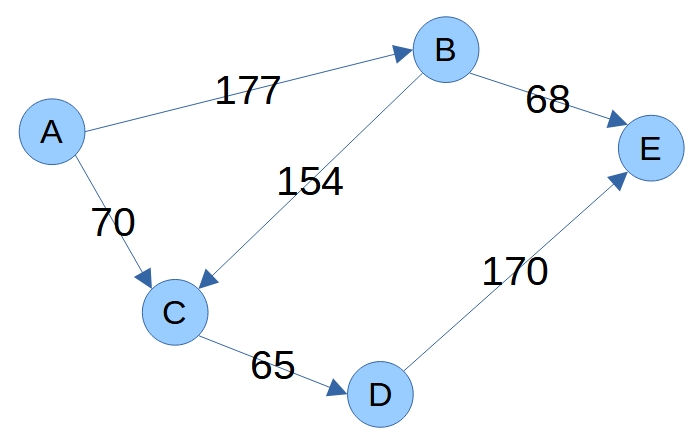
\includegraphics[width=10cm]{notes1 (1).png}\end{center}
          \textbf{Starting from node A, when node E is marked as visited, what else is on the priority queue?}\\
          \textit{E(305)}
    \item \textbf{Consider Dijkstra's algorithm, as show below.}\\
          \begin{lstlisting}[style=java]
                void printShortestPath(int source) {
                        PriorityQueue q = new PriorityQueue();
                    
                        q.enqueue(Pair(source, 0);
                        while (!q.isEmpty()) {
                            Pair p = q.deleteMin();
                    
                            if (!G[p.node].isVisited) {
                                G[p.node].isVisited = true;
                                G[p.node].dist = p.dist;
                                System.out.println("shortest distance to "" + p.node + " is " + p.dist);
                    
                                for (Edge e : G[p.node].adj) {
                                    if (!G[e.toNode].isVIsited) {
                                        q.enqueue(Pair(e.toNode, p.dist+e.cost));
                                    }
                                }
                             }
                          }
                       }
                    }
                \end{lstlisting}
          \textbf{Starting from node A, when node D is marked as visited, what else is on the priority queue?}\\
          \textit{B(177)}
    \item \textbf{Consider Dijkstra's algorithm, as show below.}\\
          \begin{lstlisting}[style=java]
                    void printShortestPath(int source) {
                        PriorityQueue q = new PriorityQueue();
                    
                        q.enqueue(Pair(source, 0);
                        while (!q.isEmpty()) {
                            Pair p = q.deleteMin();
                    
                            if (!G[p.node].isVisited) {
                                G[p.node].isVisited = true;
                                G[p.node].dist = p.dist;
                                System.out.println("shortest distance to "" + p.node + " is " + p.dist);
                    
                                for (Edge e : G[p.node].adj) {
                                    if (!G[e.toNode].isVIsited) {
                                        q.enqueue(Pair(e.toNode, p.dist+e.cost));
                                    }
                                }
                             }
                          }
                       }
                    }
                \end{lstlisting}
          \textbf{In the algorithm, why is it necessary to check if a node has been visited when pulling something off the queue?}\\
          \textit{There may be two paths to a node, so a node could get put on the queue twice}
    \item \textbf{Why do negative edge weights cause problems with Dijkstra's algorithm?}\\
          \textit{When a node is pulled off the queue, a shorter path may exist}
    \item \textbf{Dijkstra's algorithm is like a breadth first traversal, except...}\\
          \textit{Dijkstra's algorithm uses a priority queue instead of a first-in-first-out queue}
\end{enumerate}

\subsection{Network Flow}
\subsubsection{Introduction to Network Flow \& the Ford-Fulkerson algorithm}
\begin{itemize}
    \item Sink has flow in, source has flow out. Conservation Rule – In order for the assignment of flows to be valid, we must have the sum of flow coming into a vertex equal to the flow coming out of a vertex, for each vertex in the graph except the source and the sink
    \item Capacity Rule – Each flow must be less than or equal to the capacity of the edge
    \item The flow of the network is defined as the flow from the source to the sink

\end{itemize}
\subsubsection{Residual Graphs}
A residual graph is a graph derived from the original graph in the context of network flow problems. It represents the capacity that can still be added to the flow along each edge or the flow that can be removed (sent in the opposite direction). The residual graph is used to find augmenting paths to improve the flow in the network.
\paragraph{Definition:} Given a flow network G with capacities c(u, v) and a flow f(u, v), the residual graph G\_f is a graph with the same vertices as G and two types of edges:\\
-Forward edges: These have a capacity equal to the remaining capacity of the corresponding edge in the original graph (c(u, v) - f(u, v)).\\
-Backward edges: These have a capacity equal to the flow on the corresponding edge in the original graph (f(u, v)).\\
Augmenting paths: An augmenting path is a path in the residual graph where each edge has a positive residual capacity. It can be used to increase the flow in the network.
\paragraph{Augmenting Path}
Given a flow network G, an augmenting path is a simple path from the source to the sink in the corresponding residual network $G_r$. Intuitively, an augmenting path tells us how we can change the flow on certain edges in G so that we increase the overall flow from the source to the sink.
\paragraph{Ford-Fulkerson Algorithm}
The Ford-Fulkerson algorithm is a method for finding the maximum flow in a flow network by iteratively augmenting the flow along paths from the source to the sink.
\subparagraph{Steps:}
\begin{enumerate}
    \item Initialize the flow in all edges to 0.
    \item While there exists an augmenting path from the source to the sink in the residual graph (a graph that represents the remaining capacities of the edges):
          \begin{itemize}
              \item Find an augmenting path using any search method (Depth-First Search).
              \item Determine the bottleneck capacity (minimum capacity along the path).
              \item Update the flow in the original graph by sending flow along the augmenting path.
              \item Update the residual graph to reflect the updated flow.
          \end{itemize}
    \item The maximum flow is the sum of flows sent in each iteration.
\end{enumerate}

\subsubsection{Example applications of Network Flow}
Find MaxFlow algorithm
\begin{lstlisting}[style=java]
        public int findMaxFlow(int s, int tt) {
        // TODO:
        int totalFlow = 0;
        StringBuilder allPaths = new StringBuilder();

        while (hasAugmentingPath(s, t)) {
            StringBuilder path = new StringBuilder();
            int availableFlow = Integer.MAX_VALUE;
            int v = t;
            Stack<Integer> stack = new Stack<>();
            while (v != s) {
                int predecessor = vertices[v].parent;
                availableFlow = Math.min(availableFlow, getEdgeCapacity(predecessor, v));
                v = vertices[v].parent;
            }
            path.append("Flow ").append(availableFlow).append(": ");
            v = t;
            while (v != s){
                path.insert(path.indexOf(":") + 2, v + " ");
                int predecessor = vertices[v].parent;
                updateResidualGraph(predecessor, v, -availableFlow);
                updateResidualGraph(v, predecessor, availableFlow);
                v = vertices[v].parent;
            }
            path.insert(path.indexOf(":") + 2, s + " " );
            path.append("\n");
            allPaths.append(path);
            totalFlow += availableFlow;
        }
        return totalFlow;
    }
    \end{lstlisting}
\subsubsection{Edmonds-Karp algorithm}
The Edmonds-Karp algorithm is an improvement of the Ford-Fulkerson algorithm for solving the max-flow problem in a flow network. It uses BFS (Breadth-First Search) to find the augmenting paths in the residual graph.
Ford-folkerson is slow to finding optimal. Does least number of edges.
Edmonds-Karp will be sure to choose the shortest augmenting path from the source to the sink
\subsubsection{Computing the Minimum Cut}
\begin{itemize}
    \item Task: minimum number of edges to prevent flow.
\end{itemize}
\subsubsection{Computing the Maximum Flow for the Minimum Cost}
\begin{itemize}
    \item Each edge is carrying capacity: cost.v
\end{itemize}
\subsubsection{Homework 8.3}
\begin{enumerate}
    \item \textbf{What is the cost per one unit along the minimum cost route?}
          \\ What is the total cost along that route
    \item \textbf{What is the amount of flow that can be placed on the minimum cost route?} \\\textit{What ever the minimum edge value is. }
\end{enumerate}

\subsection{Minimum Spanning Trees}
A Minimum Spanning Tree (MST) is a subgraph of an undirected graph such that the subgraph spans (includes) all nodes, is connected, is acyclic, and has minimum total edge weight\\
\subsubsection{Kruskal's Algorithm}
Kruskal's Algorithm is a greedy algorithm that starts with an empty set of edges and iteratively adds edges to the MST while ensuring that the resulting graph remains a forest (a collection of trees). This one starts are the edge with the smallest capacity.
\paragraph{Steps:}
\begin{enumerate}
    \item Sort all the edges in the graph in increasing order of their weights.
    \item Initialize an empty set for the MST.
    \item Iterate through the sorted edges. For each edge (u, v):
          \\-If adding the edge (u, v) does not create a cycle, add it to the MST set.
    \item Repeat step 3 until the MST set has (V - 1) edges, where V is the number of vertices in the graph
\end{enumerate}
Kruskal's Algorithm is generally preferred for sparse graphs (few edges), as it sorts the edges, which takes O(E log E) time, and iteratively adds edges based on their weights. It is also easier to implement for disconnected graphs.
\subsubsection{Prim's Algorithm}
Prim's Algorithm is also a greedy algorithm, but it starts with an arbitrary vertex and iteratively expands the MST by adding the minimum-weight edge that connects a vertex in the MST to a vertex not in the MST.
\paragraph{Steps:}
\begin{enumerate}
    \item Choose an arbitrary vertex as the starting vertex
    \item Add all nodes reachable from this node into an empty priority queue
    \item While there are unvisited vertices, perform the following steps:
          \\ - Find the minimum-weight edge (u, v) such that u is in the visited set and v is not.
          \\ - Add edge (u, v) to the MST set and add vertex v to the visited set.
\end{enumerate}
Prim's Algorithm is more efficient for dense graphs (many edges), as it only considers edges connected to the vertices already in the MST, which can be done in O($V^2$) time using adjacency matrix representation or O(log V) time using a priority queue and adjacency list representation. It works for undirect, and weighted or unweighted graphs.

\subsection{Paths \& Circuits}
Euler paths and circuits focus on visiting every edge exactly once, while Hamilton paths and circuits focus on visiting every vertex exactly once.
\subsubsection{Introduction to Euler Paths \& Circuits}
Euler path -  visits every edge of a graph exactly once, without repeating any edges. It may repeat vertices \\
Euler circuit - a closed path that visits every edge of a graph exactly once, without repeating any edges, and starts and ends at the same node
\subsubsection{Euler Circuit Algorithm}
\subsubsection{Introduction to Hamilton Paths \& Circuits}
Hamilton Path - path that visits every vertex of a graph exactly once, without repeating any vertices
Hamilton circuit -
\subsubsection{Examples:}
\begin{center}
    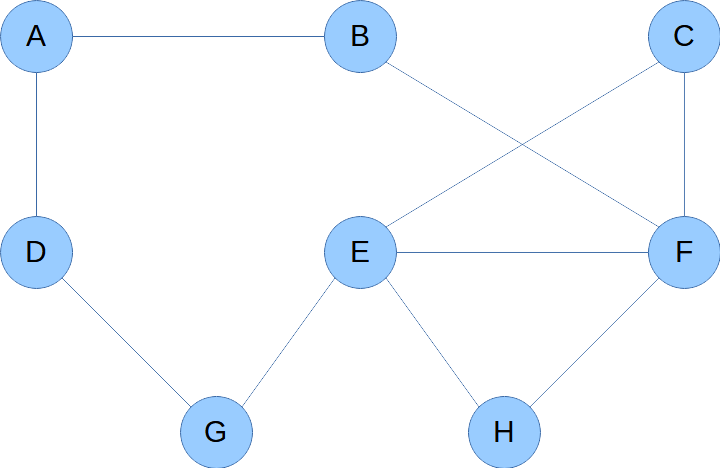
\includegraphics[width=10cm]{e1.png}\\
    Eulerian circuit\\
    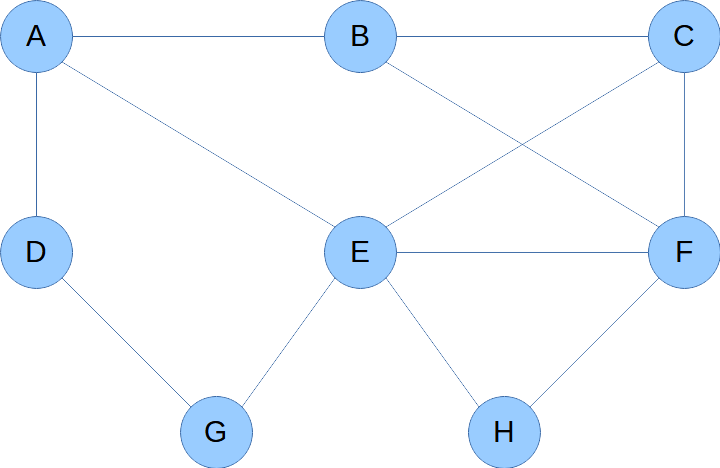
\includegraphics[width=10cm]{e2.png}\\
    Hamilotnian circuit\\
    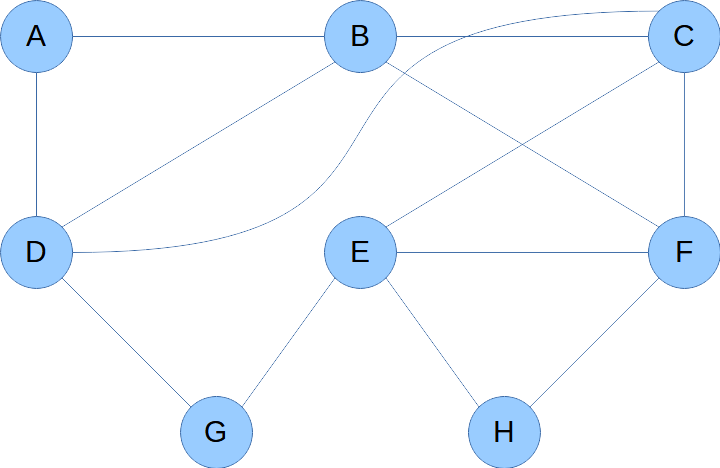
\includegraphics[width=10cm]{e3.png}\\
    Both\\
    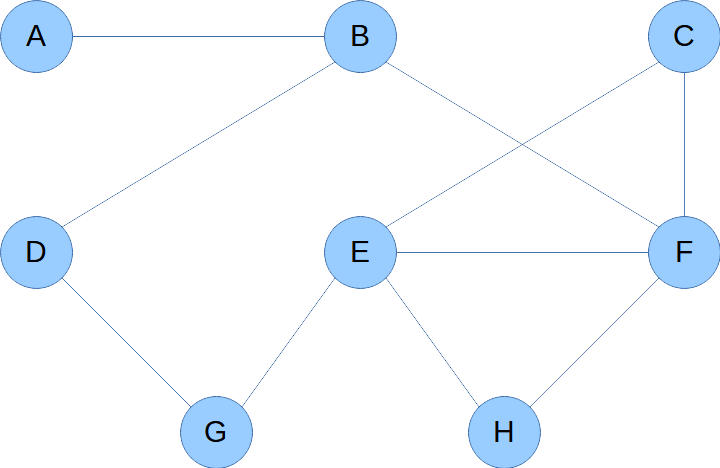
\includegraphics[width=10cm]{e4.png}\\
    Neither\\
\end{center}

\subsection{Strongly Connected Components}
\subsubsection{Finding Strongly Connected Components}
\paragraph{Step:}
\begin{enumerate}
    \item Start at desired node.
    \item Follow path by a depth first search until you've hit an already visited node, or at a end node.
    \item Once at finality node, number that.
    \item Move backwards recursively until you arrive at an unvisited node. Follow that path, repeating steps 2 and 3 until you've visited all possible adjacent nodes from the start node.
    \item Go to next start node.
    \item Repeat 1-5 until you've traversed the whole graph.
    \item Start a new tree with next highest number. Mark all nodes that can be reached. That is one connected component.
    \item Go to next highest number. Repeat until all nodes have identfied into a path.
\end{enumerate}

\subsection{Edge Types}
Tree Edge : Any edge in the tree \\
Forward Edge : Node to a successor \\
Back Edge : Node to an ancestor \\
Cross Edge : Node to an unrelated node \\
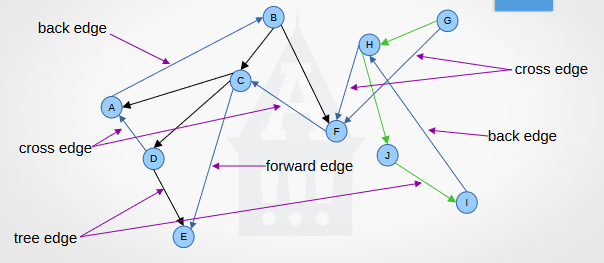
\includegraphics[width=10cm]{e5.png}
\paragraph{Questions}
\begin{enumerate}
    \item \textbf{The object of the Kevin Bacon game is to link a movie actor to Kevin Bacon via shared movie roles.  The minimum number of links is an actor's Bacon number.  For instance, Tom Hanks has a Bacon number of 1 as he was in Apollo 13 with Kevin Bacon.  Sally Field has a Bacon number of 2, because she was in Forrest Gump with Tom Hanks who was in Apollo 13 with Kevin Bacon. Forming this as a graph problem, what are the edges?}\\
          \textit{ Been in a movie with }
    \item \textbf{Finding an actor's Bacon number is what kind of problem?}\\\textit{Shortest path}
    \item \textbf{A student needs to take a certain number of classes to graduate, and these courses have prerequisites that must be followed.  Assume that every class is offered every semester and that a student can take an unlimited number of courses.  Given a list a courses that a student wants to take and their prerequisites, compute a schedule that requires the minimum number of semesters. Which algorithm would be most useful?}\\
          \textit{topologicalOrdering}
    \item \textbf{Suppose that a maze exists, but may or may not be solvable.  You want to determine if the maze is solvable. Which algorithm will be most helpful?}\\ \textit{Union Find}
    \item \textbf{We have two sets: People and Candy Bars.  A perfect matching is a matching in which every item in the People set is paired with an item in the Candy Bar set, such that all Candy Bars are matched. Which algorithm will be most helpful?} \\
          \textit{Maximum Flow}
    \item \textbf{We need to build a connected network.  We have a limited set of possible routes, and we want to select a subset that will make our network (e.g., electrical grid, computer network)  connected at the lowest cost. Which algorithm is most helpful?}\\ \textit{Minimal Spanning Tree }
\end{enumerate}

\subsection{Biconnected Graphs}
An articulation point is a node whose removal does disconnect the graph.

\subsection{Hard vs. Easy Problems}
\paragraph{Vertex Cover}
A vertex cover of an undirected graph is a subset of vertices such that it includes at least one endpoint of every edge of the graph. The goal is to find the minimum vertex cover, which is the smallest possible subset of vertices that still satisfies this property.
\subparagraph{Steps:}
\begin{enumerate}
    \item Start with an empty set for the vertex cover.
    \item While there are uncovered edges, perform the following steps:
          \begin{itemize}
              \item Choose an uncovered edge (u, v).
              \item Add both vertices u and v to the vertex cover set.
              \item Remove all edges incident to either u or v from the graph (as they are now covered).
          \end{itemize}
    \item The resulting vertex cover set is an approximation of the minimum vertex cover. It does not guarentee  an optimal solution.
\end{enumerate}

\section{Unit 9: Introduction to Algorithm Design}
\subsection{Introductinon to Dynamic Programming}
\paragraph{Greed Algorithms}
Greedy algorithms are a class of algorithms that make locally optimal choices at each step, with the hope that these choices will lead to a globally optimal solution. These algorithms are generally simple to implement and have good performance for certain problems. However, they may not always provide optimal solutions.
\subparagraph{Memorizing}
Solving the repeated sub-problem compute problem. An optimization technique used primarily to speed up computer programs by storing the results of
expensive function calls and returning the cached result when the same inputs occur again.\\
Example: Fibonacci Sequence - Calculating the nth Fibonacci number using naive recursion results in exponential time complexity. Using memoization, the computed values of Fibonacci numbers are stored in a cache (e.g., an array or dictionary), and when the function is called again with the same input, the cached result is returned instead of re-computing the value, reducing the time complexity to linear.
\subparagraph{Dynamic Programming}
Dynamic programming is a technique used to solve problems by breaking them down into smaller, overlapping subproblems and solving them in a bottom-up manner. The solutions to subproblems are stored in a table to avoid redundant computations, which reduces time complexity. Dynamic programming is particularly useful for optimization problems, and it guarantees an optimal solution when applicable.\\
\begin{itemize}
    \item Overlapping subproblems: Problems that can be broken down into smaller subproblems that are solved multiple times.
    \item Optimal substructure: The optimal solution to the problem can be constructed from optimal solutions of its subproblems.
    \item Bottom-up approach: Solve smaller subproblems first and use their solutions to construct solutions for larger subproblems.
\end{itemize}
Example: Longest Common Subsequence (LCS) - The LCS problem involves finding the longest subsequence that is common to two input sequences. Dynamic programming can be applied by creating a table to store the LCS length for each pair of input characters, using a bottom-up approach to fill the table, and finally constructing the LCS from the table.\\
Example: The Making Change problem involves finding the minimum number of coins required to make a given amount of change. A greedy algorithm can solve the problem for certain coin systems (e.g., US coins) by always choosing the largest denomination coin that is less than or equal to the remaining change. However, for arbitrary coin systems, a dynamic programming approach is needed to find the optimal solution, by constructing a table of minimum coins needed for all amounts from 1 to the target amount.

\section{Additional Graphics}

\end{document}